\section{Dynamic time warping}

\subsection[short]{Introduction}

Given a time series of three-dimensional unknown vector data points, we would like to predict the sketch represented by these points. In order to do this, we used a K-Nearest Neighbors approach where we find the $k$ most similar time series in the dataset and use the most represented target value among the $k$ time series to use it as the prediction output.

To find the $k$ most similar time series, we use a distance function as the similarity measure. However, we cannot use the often used euclidean distance as it produces pessimistic results when dealing with time series of different lengths (a typical example is two same time series with one shifted on the time axis).

Dynamic time warping --- a often used technique in speech recognition problem --- is a solution to this problem, it finds the optimum alignment between two time series by "warping" non-linearly a time series stretching or shrinking its time axis. Once we found the optimal alignment, we can determine the similarity between these twos.

Let $s = (s_1, \dots, s_n)$ and $t = (t_1, \dots, t_m)$ be two time series of length $n$ and $m$ respectively where $s_i$, $t_j$ are the position vector $\in \R^3$ for $i = 1,\dots,n$ and $j = 1,\dots,m$. We define a warping of order $n \times m$ as a sequence of $k$ points $x = (x_1, \dots, x_k)$ where $x_l = (i_l, j_l) \in [1, n] \times [1, m]$. Each points $x_l$ of the path aligns the vector $s_{i_l}$ with the vector $t_{i_l}$.

The following constraints apply,
\begin{itemize}
	\item \textbf{boundary conditions}: $x_1 = (1, 1)$ and $x_k = (n, m)$. This ensures that every index of the time series are used in the warp path.
	\item \textbf{locality}: $x_{l+1} - x_{l} \in \set{(1,0),(1,1),(0,1)}, \quad \forall l \in [1, k-1]$.
\end{itemize}

The locality condition implies a monotonicity condition: $s_1 \leq \dots \leq s_n$ and $t_1 \leq \dots \leq s_m$. This monotonicity implies that the lines representing the warp path do not overlap.

Among all the warping path we can construct, want to find the optimal warping path $x^{\ast}$ that consists in the warping path that minimizes the square root of the following cost given for any warping path $x$,
\begin{equation}
	C_x(s, t) = \sum_{l=0}^{k} ||s_{i_l} - t_{j_l} ||^2_2
\end{equation}

We can then compute the dtw distance by computing the total cost of the warping path $x^{\ast}$. 

In practice, to find the optimal path, we use a dynamic programming approach which consists in the following algorithm,
\begin{enumerate}
	\item We define a distance matrix $D \in \R^{n \times m}$ where $D_{i,j}$ is the minimum-distance for the warping path between $s' = (s_1,\dots,s_i)$ and $t' = (t_1,\dots,t_j)$.
	\item Each entry is computed by using the following recursion formula,
	\begin{equation}
		D_{i,j} = ||s_i - r_j|| - \min{(D_{i-1,j}, D_{i-1,j-1}, D_{i,j-1})}
	\end{equation}
	with the initial condition $D_{1,1} = 0$
	\item The entry $D(n, m)$ contains the minimum-distance for the warping path between $s$ and $t$.
\end{enumerate}

This algorithm has $\mathcal{O}(nm)$ time complexity. We can however speed up the algorithm by applying \textbf{contraints} that consists in limiting the number of cells that are evaluated in the distance matrix (e.g. using a Sakoe-Chiba Band window\footnote{In a nutshell, this window assumes that the best path will not stray too far away from the main diagonal of the distance matrix.}) and \textbf{data abstraction} that consists in performing the algorithm on a reduced representation of the data (\cite{Salvador_Chan}). Instead of running the algorithm on the full distance matrix, we reduce the size of the time series which implies that the number of cells in the distance matrix are reduced. Once the warping path is found on this low-resolution matrix, we map it back to a higher-resolution matrix. This projected path is used as an initial guess for a new warping path on this new distance matrix. In other words, the projected path is refined on the higher-resolution matrix by making \textbf{local adjustments}\footnote{These local adjustments can be controlled through a radius parameter that controls the number of cells that will be evaluated around the path.} which implies that this matrix is only filled in the neighborhood of the projected path. This results in a algorithm with linear time complexity since the warping path grows linearly with the size of the time series. 

Research have shown that using a single neighbor in the KNN algorithm gives the best results (\cite{Mitsa_2010}). Moreover, trying different combination of number of neighbors and radius hyperparameters, we notices that a good trade-off between efficiency and rapidity was not only obtained with a single neighbor but also with a radius of 1.

% This can be improved by the use of a window of size $r > 0$ that will constrain the amount of warping allowed. In particular, it restrains the distance in the time axis that a point $s_i$, $i = 1,\dots,n$ can be mapped to in $t$.

% We can use the so-called \textit{"Sakoe-Chiba Band"} window which assumes that the best path will not stray too far away from the main diagonal of the distance matrix. 
% Let $w$ be the window size, the window constraint implies the following,
% \begin{align*}
% 	j - w \leq i \leq j + w
% \end{align*}
% where $i$ and $j$ are two points aligning in $s$ and $t$ respectively. The number of cells that needs to be computed in the distance matrix is therefore reduced. However, this constraints does not work so well if we have time series stopping at radically different time. For such time series, the warping path can stray far away from the linear one implying the need to fill (almost) the whole distance matrix.

\subsection{Results}

\subsubsection{User-independent cross-validation}

In the user-independent cross-validation, for the first domain, we get a mean accuracy of $0.743$ with a large standard deviation of $0.146$. Interestingly, looking at the confusion matrices for the different splits, we notice a lof of misclassifications for the last split. It could be that one user has a very poor handwritting compared to the others so that our system is not properly trained to recognize the shapes from this split.

\begin{figure}[H]
	\centering
	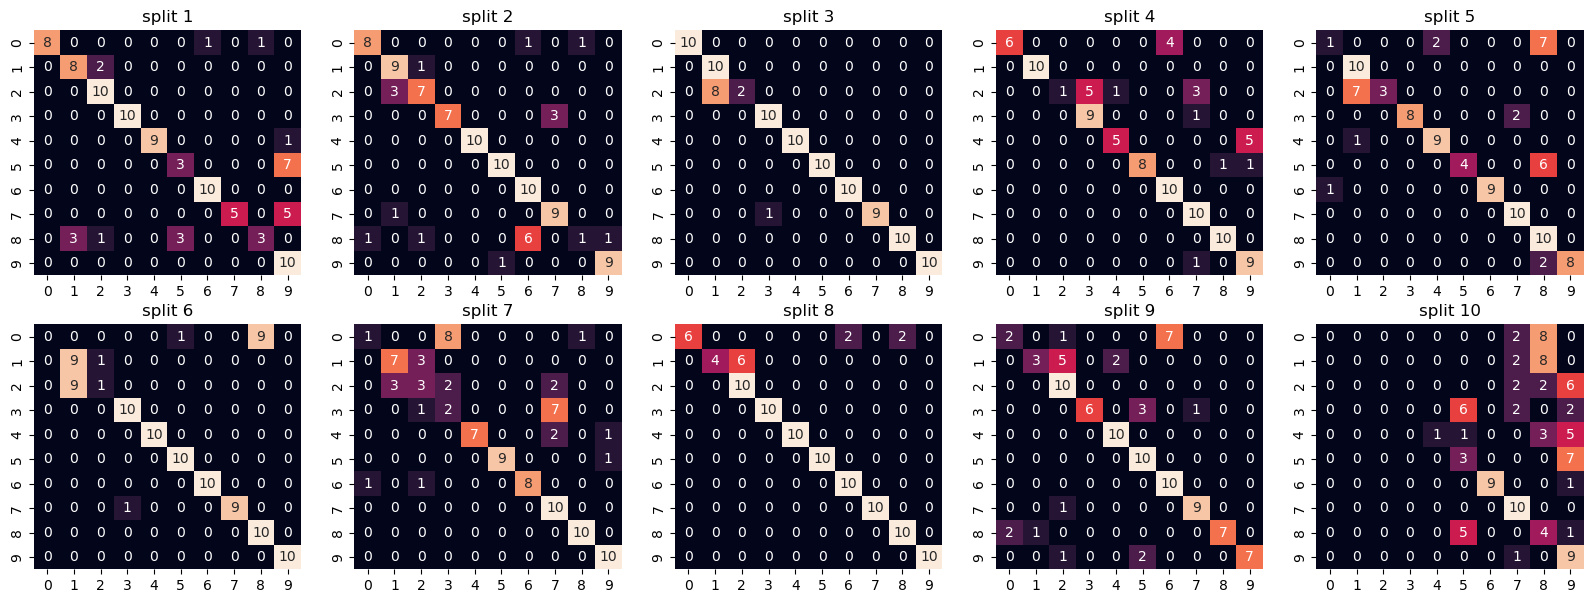
\includegraphics{figures/dtw/domain01/cm_dtw_d1_uindep.png}
	\caption{Confusion matrices of the different splits for the domain 1 using fast DTW algorithm (user independent cross-validation)}
	\label{fig:cm-dtw-d1-uindep}
\end{figure}

For the third domain however, we get a mean accuracy of $0.853$ with still a large standard deviation of $0.117$. It was pretty much unexcepted as this domain contains more complex sketches than simple numbers. Here it is the split nine that contains a lot of missclassifications. The same reason as above could explain it.

\begin{figure}[H]
	\centering
	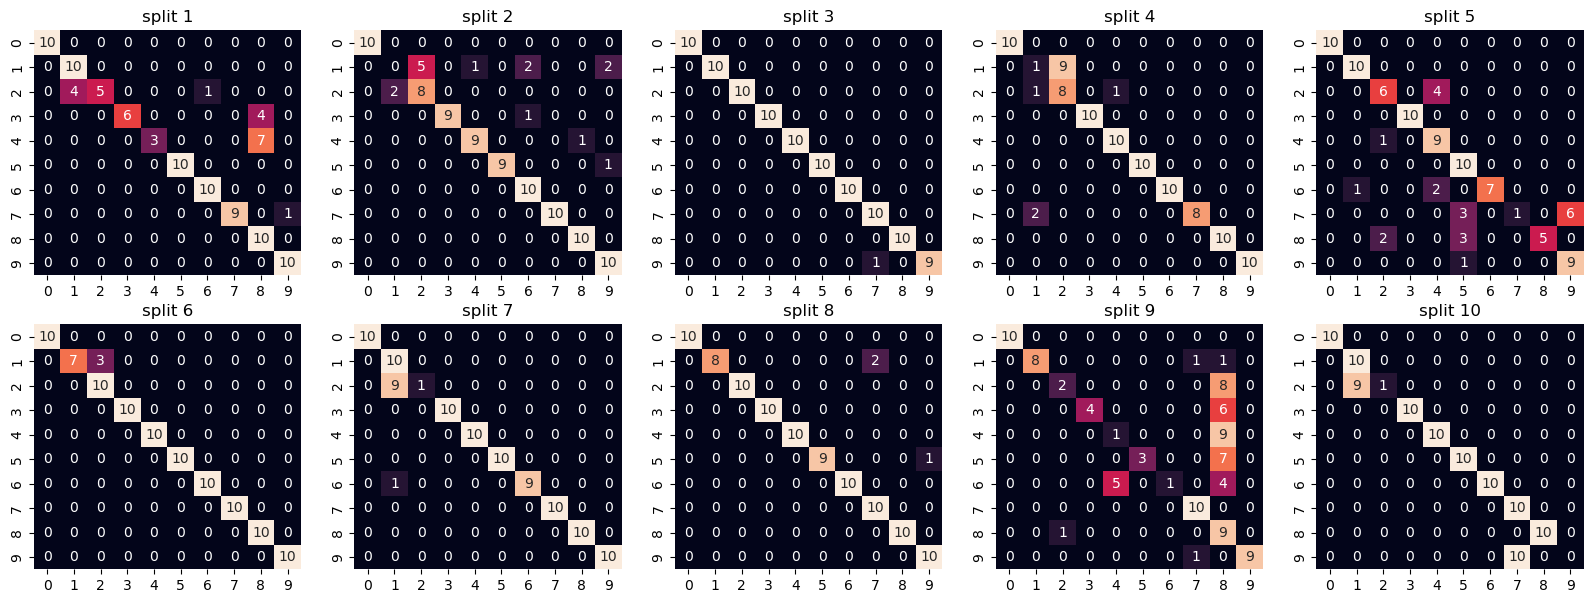
\includegraphics{figures/dtw/domain03/cm_dtw_d3_uindep.png}
	\caption{Confusion matrices of the different splits for the domain 3 using fast DTW algorithm (user independent cross-validation)}
	\label{fig:cm-dtw-d3-uindep}
\end{figure}

\subsubsection{User-dependent cross-validation}

In the user-dependentent cross-validation, we get far more better results. For the first domain, our classifier is almost perfect with a mean accuracy of $0.99$ and a standard deviation of $0.009$. This makes sense to get better results since the data from all the users are used to train the algorithm.

\begin{figure}[H]
	\centering
	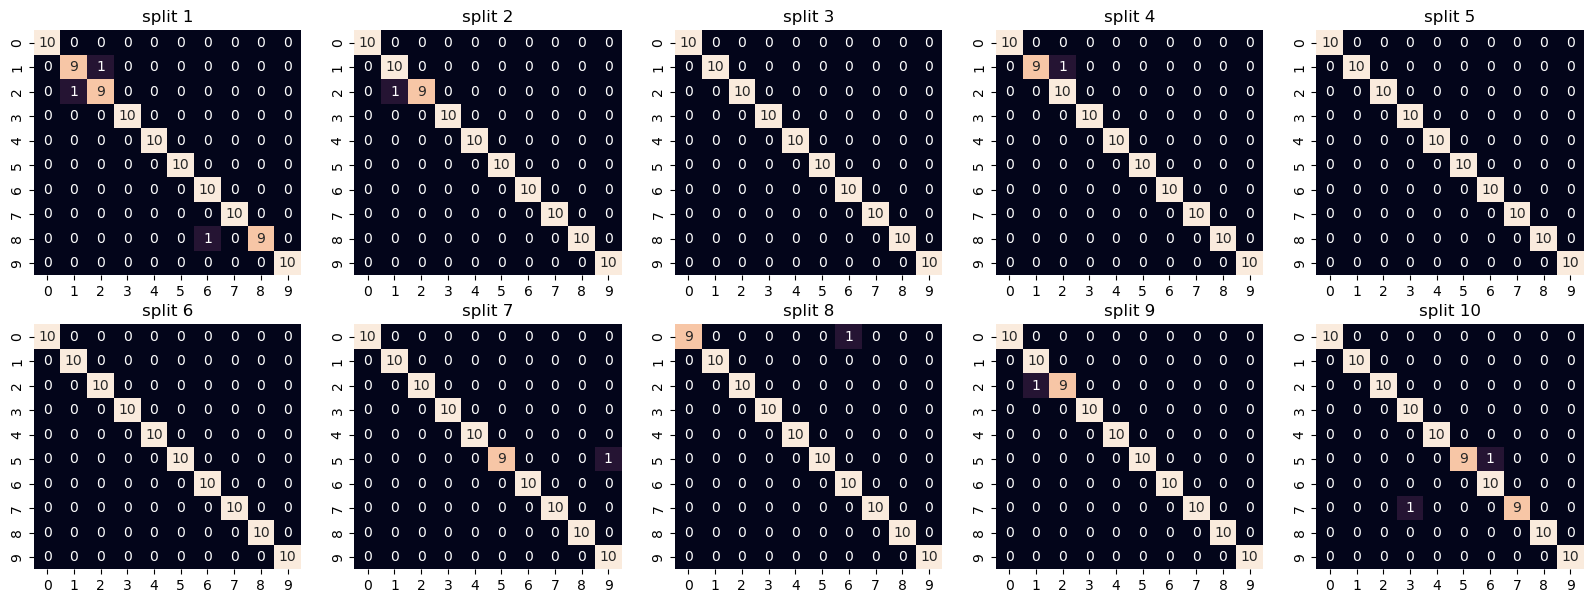
\includegraphics{figures/dtw/domain01/cm_dtw_d1_udep.png}
	\caption{Confusion matrices of the different splits for the domain 1 using fast DTW algorithm (user dependent cross-validation)}
	\label{fig:cm-dtw-d1-udep}
\end{figure}

For the third domain, we have a mean accuracy of $0.997$ and a standard deviation of $0.005$. This is still impressive.

\begin{figure}[H]
	\centering
	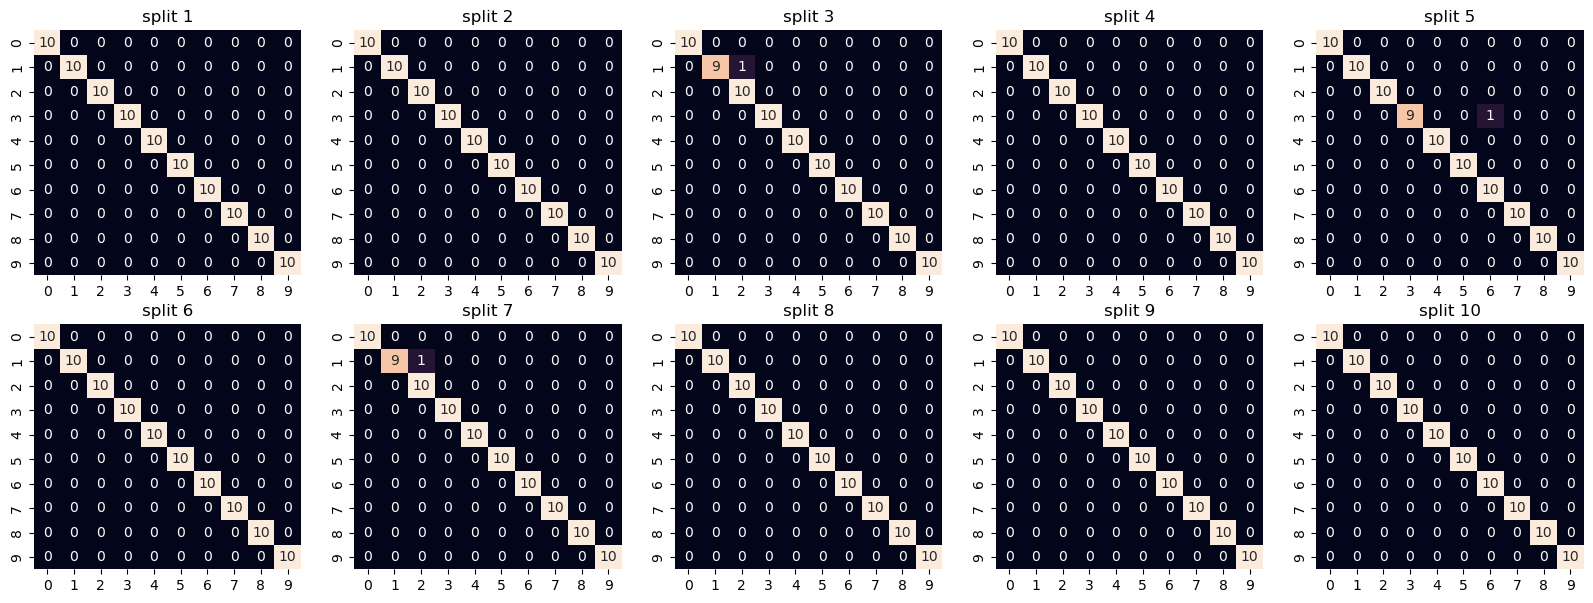
\includegraphics{figures/dtw/domain03/cm_dtw_d3_udep.png}
	\caption{Confusion matrices of the different splits for the domain 3 using fast DTW algorithm (user dependent cross-validation)}
	\label{fig:cm-dtw-d3-udep}
\end{figure}